\chapter{Appendix}\label{chap:appendix}
This chapter shows the raw images acquired with the aquarium and Aeolotron setup and their respective measurement conditions. The shown figures are meant to demonstrate the difference between the different bubble concentrations.

\begin{figure}
	\centering
	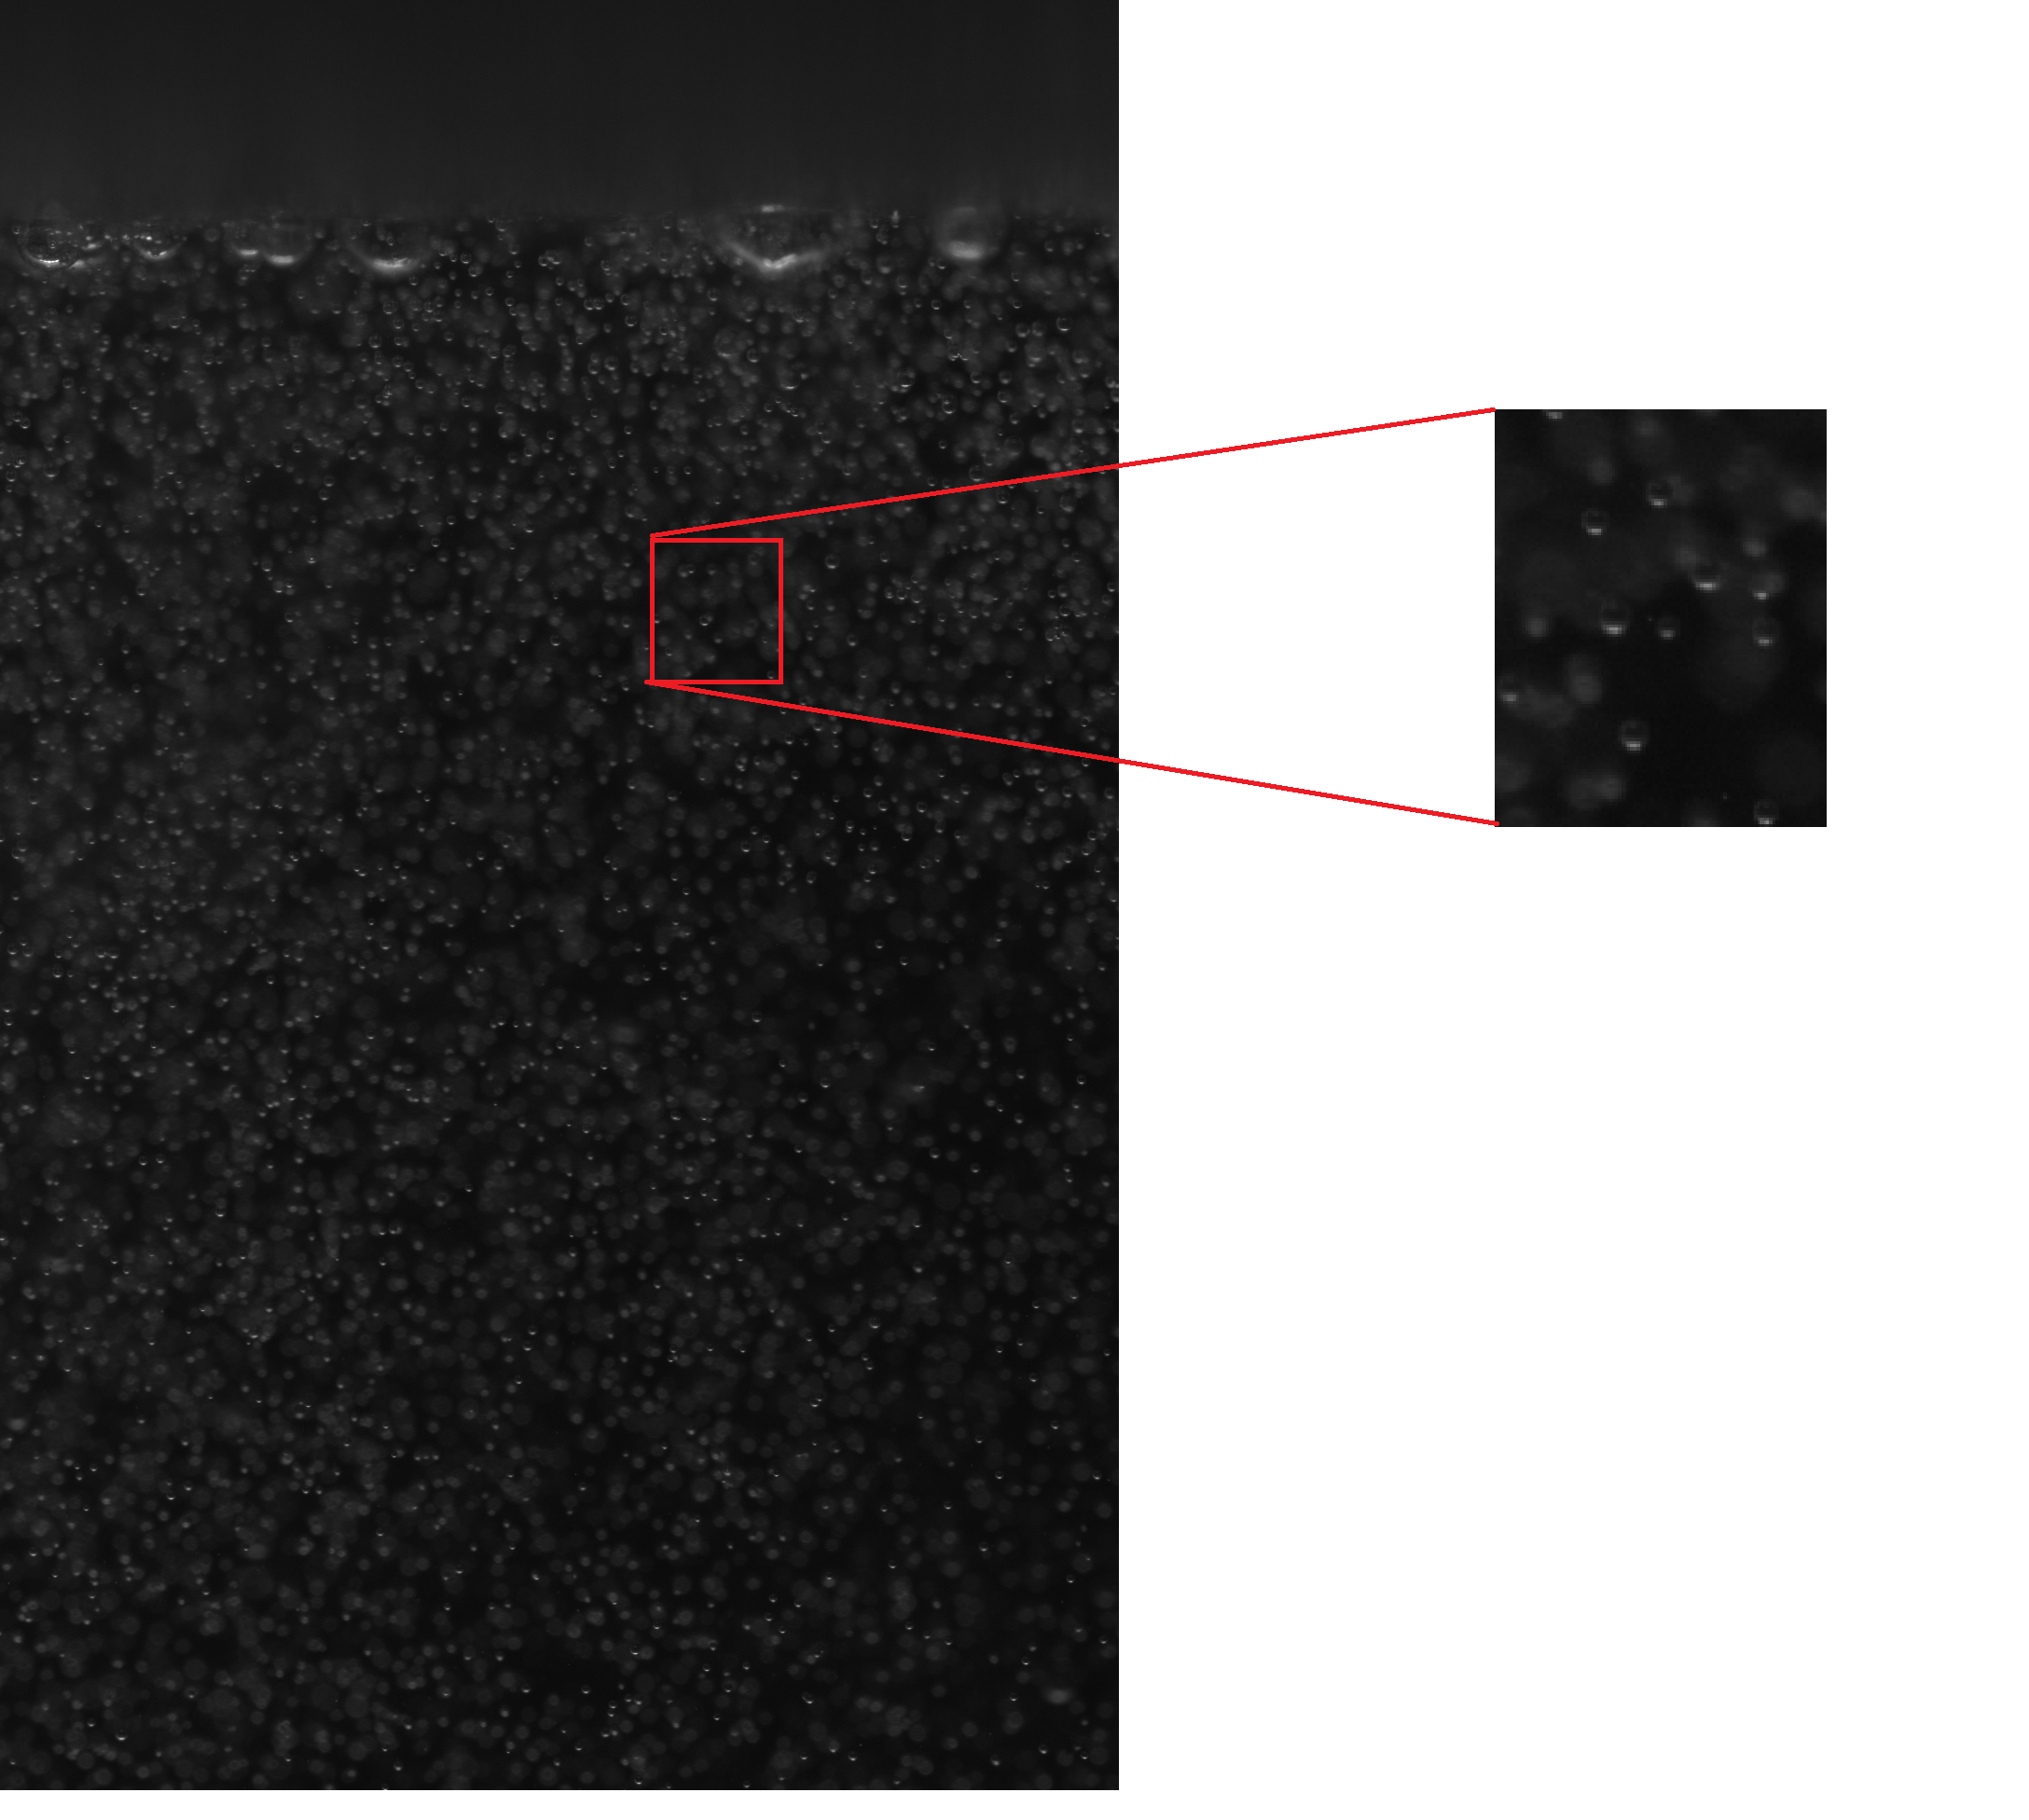
\includegraphics[scale=0.4]{images/aquarium_result_surf.png}
	\caption{Image captured close to the water surface with the aquarium setup. The cutoff line at the upper part of the image is the water surface.  
	Most bubbles show the expected two peaks, except for those very close to the water surface, where bubble curvatures is also visible. Settings are the same as in table \ref{tab:aquarium_param} with an airflow of 1.8\,LPM}
\end{figure}

\begin{figure}
	\centering
	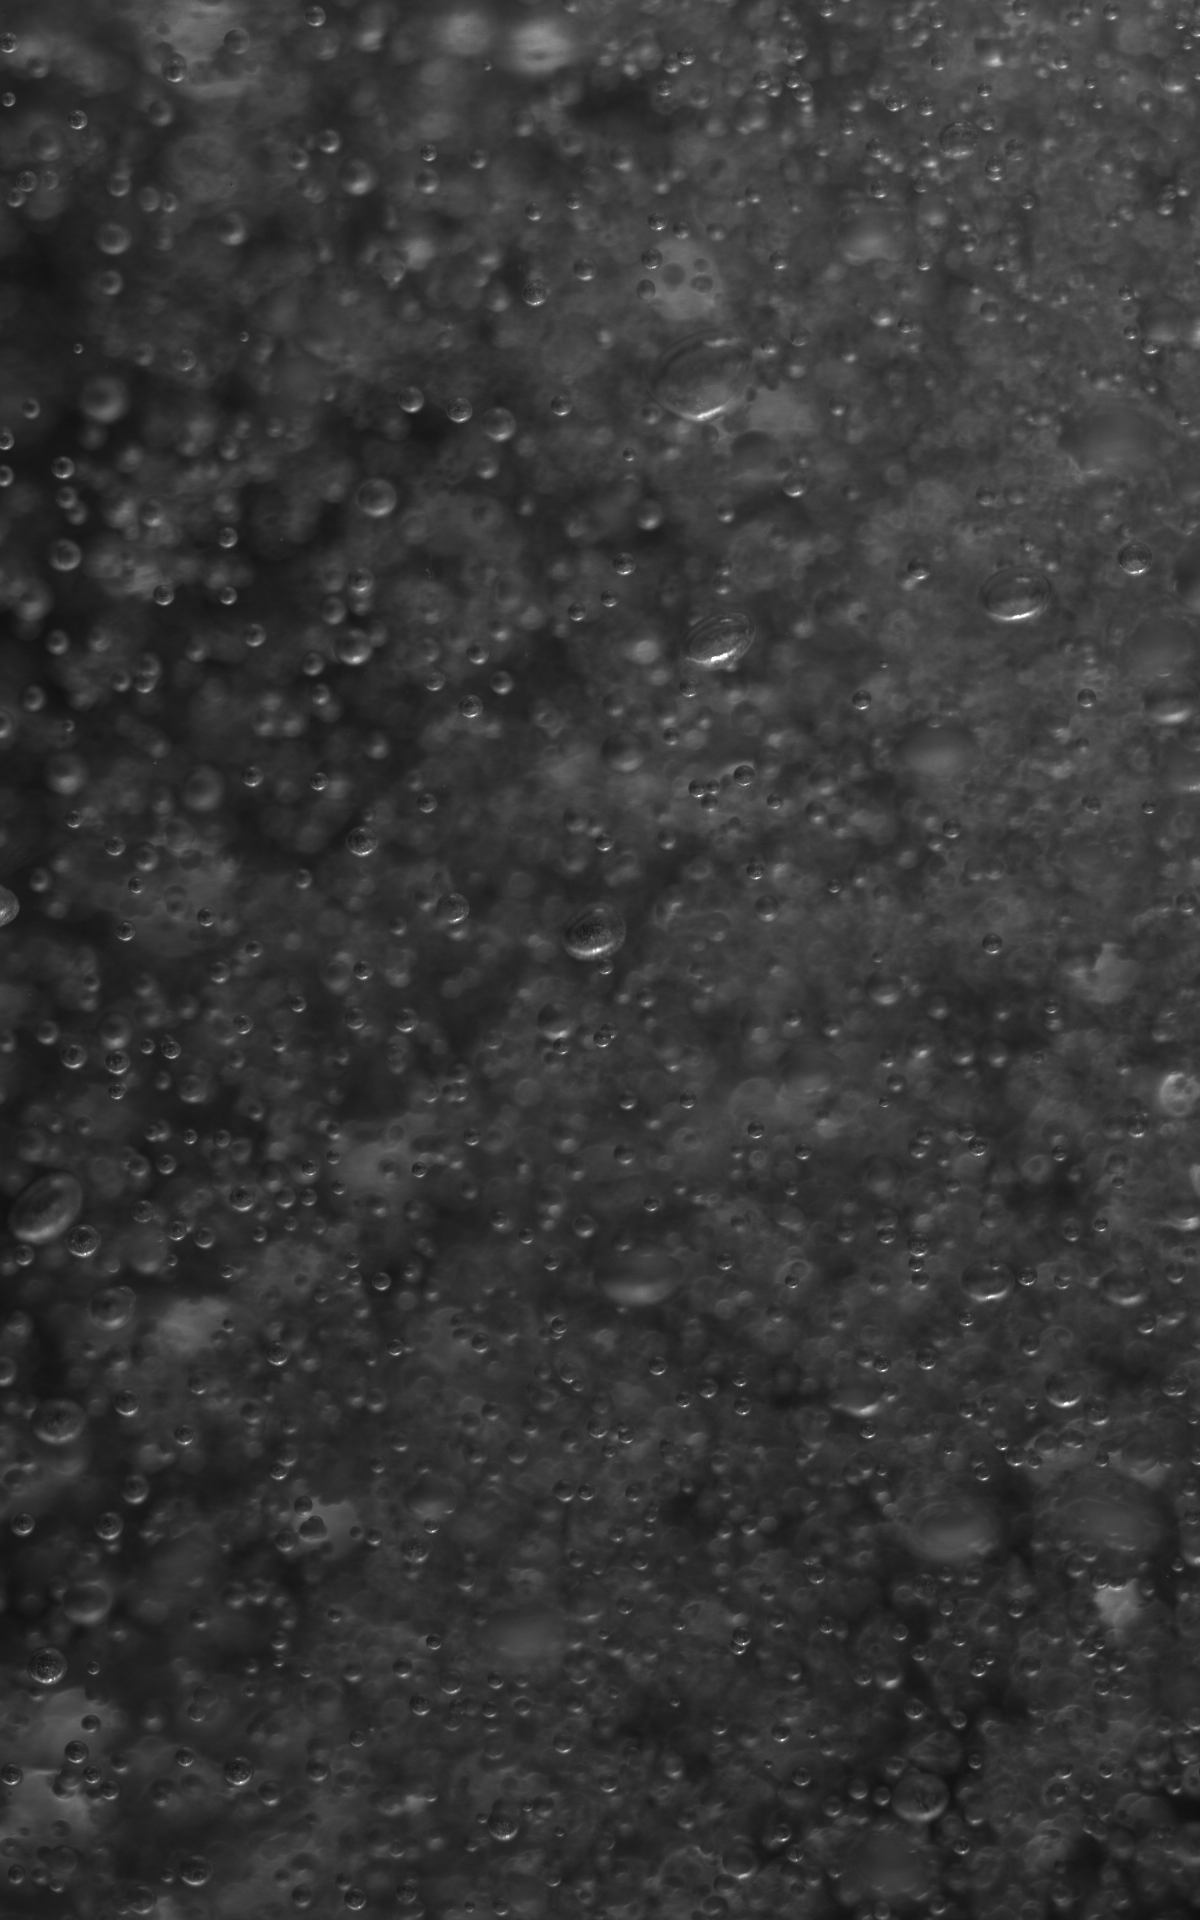
\includegraphics[scale=0.3]{images/aquarium_result_high_conc.jpg}
	\caption{Image with high bubble concentration at aquarium setup using a bubble generator. The image was positioned at around 20\,cm below the water surface and 40\,cm above the bubble generator. A high variation in bubble sizes can be observed. The background is also much brighter than in the previous image. }
\end{figure}


\begin{figure}
	\centering
	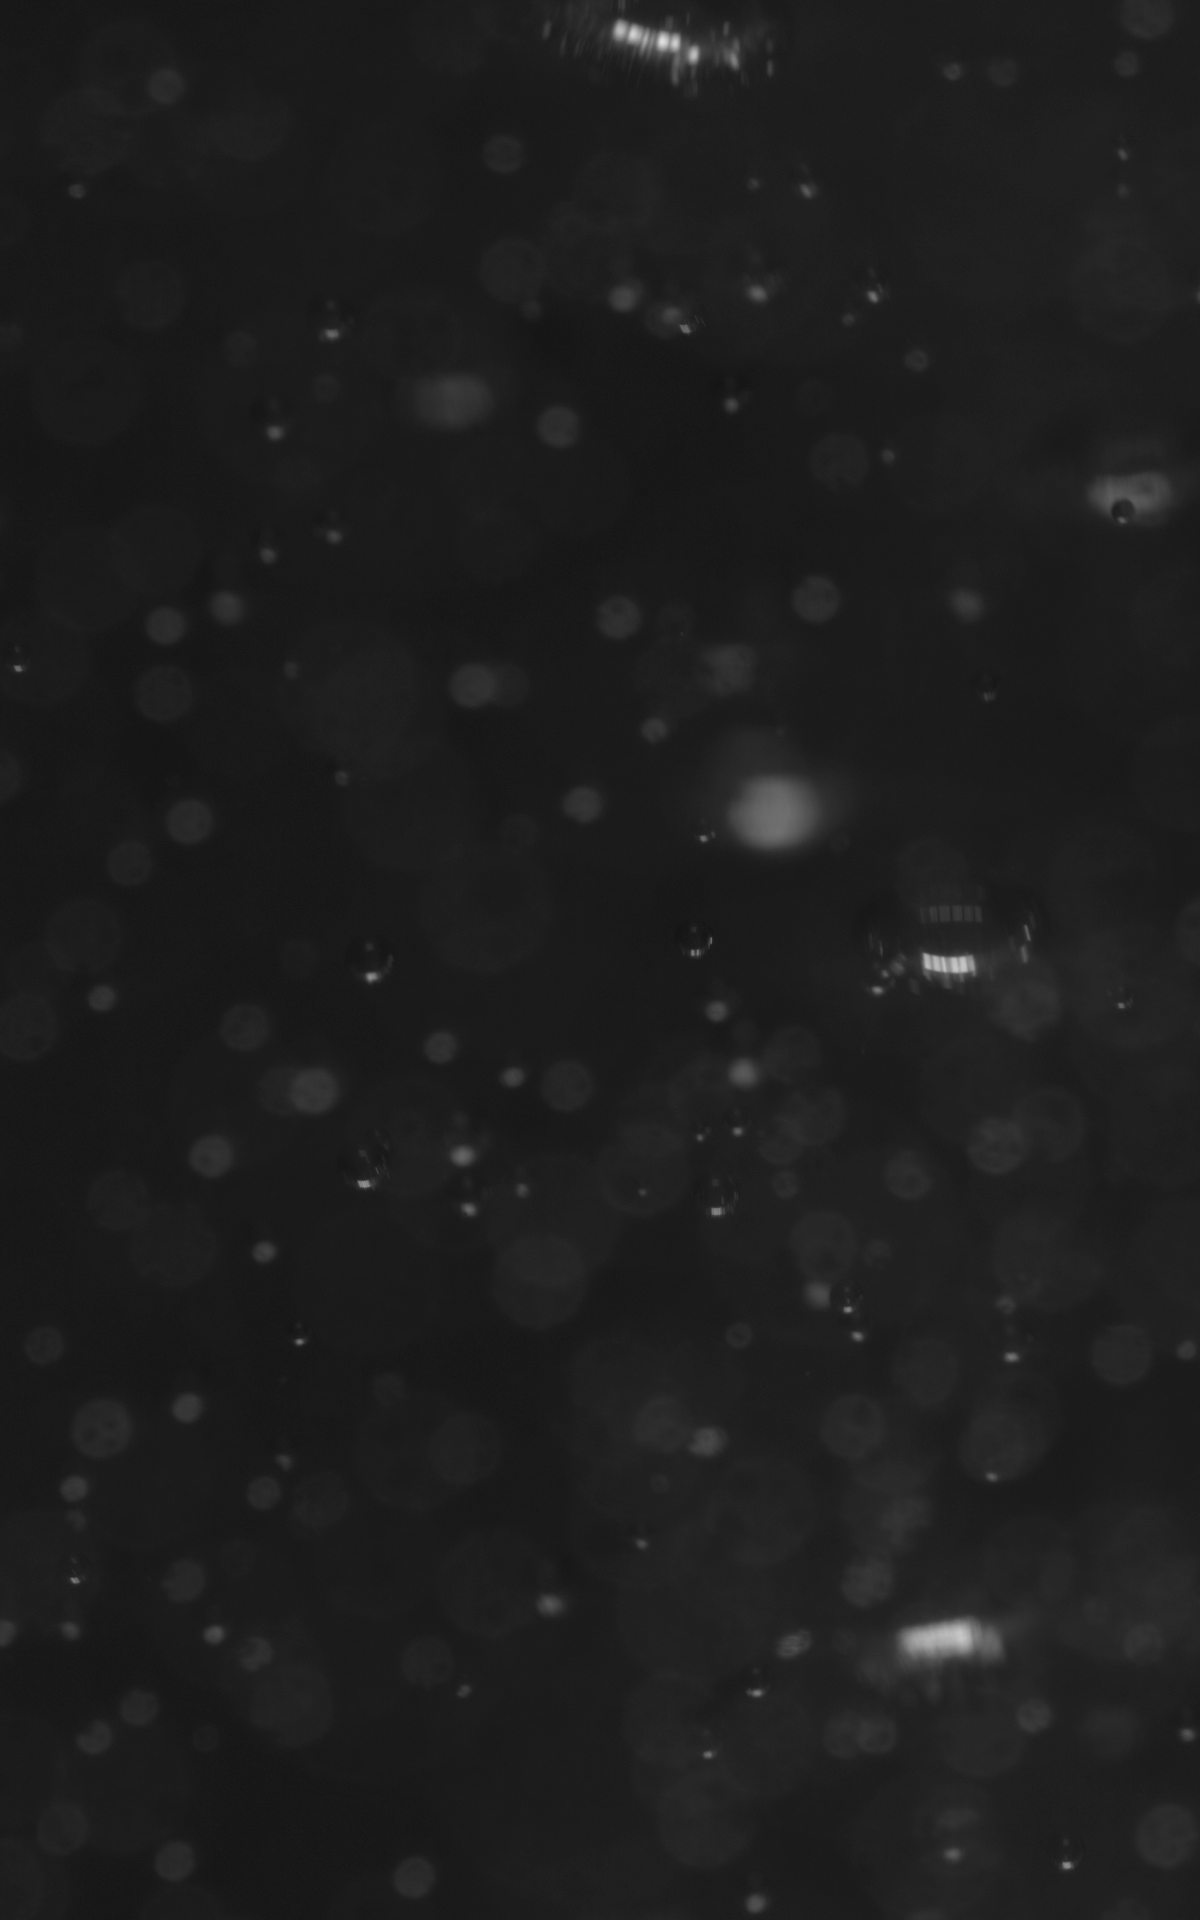
\includegraphics[scale=0.3]{images/aeolotron_result_raw.png}
	\caption{Image from Aeolotron setup with low bubble concentrations. Motion blur can be observed for fast moving large bubbles. The camera was positioned at about 5\,cm below the water surface. Settings are described in table \ref{tab:aeolotron_setup}.}
\end{figure}